This bachelor thesis aims to discuss the main maze exploration algorithms and then propose a method where multi-agents must find the maze solution without any type of communication, only working with coordinated and deterministic distributions to guide their behaviors. The main challenge of this research is to find a distributed exploration approach with total communication restriction since an agent's partial knowledge cannot be shared with another agent and, at the same time, a single agent must avoid repeating a branch of another agent. The proposed maze structure abstraction is a traditional regular grid that can be generalized into graphs.

This report is the initial part of the bachelor's thesis, and this chapter intends to introduce the general concept of the related thesis and present the motivation (Section \ref{section_intro_motivation}), the related work (Section \ref{section_intro_relatedwork}), and the main definitions about maze-solving algorithms (Section \ref{section_intro_definitions}).

\section{Motivation}
\label{section_intro_motivation}
Graph exploration has been the target of studies since Leonhard Euler proved that Seven Bridges of K�nigsberg \cite{ShieldsR2012} has no solution. It has been researched not only in academia but also in the industry due to several practical applications, like airline scheduling, planning path on maps, search engine algorithms, social media marketing, Internet routing protocols, and robotics.

Specifically in robotics, graph exploration can be used to explore a maze with a single agent through a bunch of traditional algorithms: random mouse, wall follower, Tr�maux, etc \cite{Sadik2010}. And it can be useful to guide many real-life problems such as search in nuclear plant disasters, burning buildings, and extraterrestrial environments. In these previous examples, the multi-agent exploration potentially can speed up the exploration, despite of it will be ineffective if different agents explore the same portions of the graph. Recent studies have explored multi-agent maze-solving algorithms as seen in the Multi-Agent Maze Exploration paper \cite{KivelevitchCohen2010}, where authors proposed a Tarry's algorithm generalization. It is important to emphasize that maze-solving algorithms consider that the structure is unknown.

%ERRADO: , and then traditional search algorithms, such as Dijkstra and A*, cannot be used to solve the maze.

Traditional multi-agent maze exploration approaches is based on internal communication between agents, where each agent knows about visited cells by another agent. It avoids a second exploration in a useless path and thus it decreases computational costs. However, there are some real situations where communication is limited or impossible, such as deep sea exploration, search in large wall structures, or search with low energy-based autonomous agents. 

However, the zero-communication approach between agents have not been concretely found in the literature despite it may have real applications and may guide search plans in real-world problems. In order to explore it, this work presents some ways to achieve the solution of a maze based on agents without communication, that might be generalized to graph exploration algorithms.

\section{Related work}
\label{section_intro_relatedwork}
Multi-agent cooperative system approaches are common in literature, especially when it comes from robotics researches. In the context of communicable agents, mainly in robotics, this chapter presents some related works.

\citen{MataricMJ1995} established common properties across different scenarios of mobile multi-agent interactions, such as dispersion - ``the ability of a group of agents to spread out in order to establish and maintain some minimum interagent distance'' -, aggregation - ``the ability of a group of agents to gather in order to establish and maintain some maximum interagent distance'' -, homing - ``the ability of an agent to find a particular region or location'' -, etc. The author proposes a synthetic structure in order to abstract different types of interagent basis behaviors.

\citen{Burgard2005} pointed out that an exploration group of robots takes several advantages over single agent exploration, despite a coordinating group might introduce redundancy. The authors present an algorithm to efficiently explore an environment by mobile and autonomous robots within a centralized communication range. These coordinated robots can completely cover the environment in a significantly reduced time compared to other related approaches cited in the article. However, this bachelor thesis intends to study a different technique based on zero-communication range. 

\citen{Sadik2010} presents, as seen in the title of the paper, a comprehensive and comparative study of maze-solving algorithms techniques by implementing graph theory. The research is delimited in the ``Micromouse competition'' context, which is a famous maze competition that has been performed worldwide since late 1970s. The authors compared maze-solving methods based on graph theory algorithms, such as DFS (Depth First Search) and BFS (Breath First Search) flood-fill, to common algorithms in the ``Micromouse'' context, such as Wall Follower. They concluded that, despite graph theory algorithms demands higher computational complexity, they are more proficient compared to related algorithms that doesn't use graph representation, and only make decisions relied on the neighborhood.

Based around maze-solving algorithms, \citen{KivelevitchCohen2010} proposed a generalization of Tarry's algorithm, but the new approach is that all visited cells of the maze are known by each agent, since each agent shares its knowledge with all the others. In that sense, each one holds an dynamic map of the maze excluding redundant information, allowing information sharing. The authors presents in the article the performance of the proposed solution, where a group of virtual coordinate agents is required to find the goal without an \textit{a priori} knowledge of the maze, so-called ``maze exploration''.

\citen{Beisel2014}, similarly to aforementioned, worked in simulation and mathematical analysis for strategies related to cooperative autonomous robots, that can share messages with each other to exit a maze. The author concluded that a cooperative approach might result in significant performance improvements compared to uncooperative and uncoordinated robots.

\section{Definitions}
\label{section_intro_definitions}
Mainly considering these previous references, this chapter intends to define common terms about maze-solving algorithms, graph theory, and mathematical tools that were useful to abstract the proposed solution. Furthermore, it intends to clarify the approach domain of this work.

\subsection{Graph}
\label{section_definitions_graph}
Graph theory has been used in various real-life applications, such as in biology, social sciences, engineering, computer science, etc. \citen{Manber1989} establishes that a graph $G=(V,E)$ consists of a set $V$ of vertices (also called nodes), and a set $E$ of edges. Each edge corresponds to a pair of vertices, and represents relationships among the vertices. A graph can be directed or undirected. The edges in a directed graph are ordered pairs, i.e., the order of the edge connection between two vertices is important. On the other hand, the edges in an undirected graph are unordered pairs, i.e., the order of the edge connection between two vertices is not important. The author gives an example: a graph may represent a set of people, and the edges may connect any two persons who know each other. Moreover, he discuss several computational problems in terms of graphs, where he describes famous graph exploration algorithms, such as DFS (Depth First Search) and BFS (Breath First Search). Please check \citen{Manber1989} for more details.

\citen{Manber1989} works with some representations of graphs in his book. One of representations is the adjacency list of a graph, that is described by an array of lists. In the adjacency list representation, each vertex is associated with a linked list consisting of all the edges adjacent to this vertex. Supposing that $|V|=n$, the adjacency list will have $n$ linked lists. In the case of this work, graphs are always undirected, therefore, if the linked list $i$ of a vertex $v_{i}$ has a vertex $v_{j}$, the linked list $j$ will have the vertex $v_{i}$.

It is worth to mention that there is a subdomain of graph data type called tree. A tree is also an abstract data type, which can be represented topologically as a hierarchical structure of nodes. \citen{Manber1989} indicates that, in a tree, it is possible to hierarchize all the edges from the root (the head node in terms of tree hierarchy), and hence trees are sometimes called rooted trees.

From Section \ref{section_models_maze_graph}, a perspective of a maze from a tree and a graph topologies will be explored.


\subsection{Maze}
This report define a maze at the same perspective presented in \citen{KivelevitchCohen2010}. A maze is a n-dimensional gridded space of any size, usually rectangular. The gridded space is composed by a set of cells, while a cell is the elementary item of a maze, defined as a delimited n-dimensional space. Cells might be connected or not connected to another adjacent cell, separated by a ``wall'' in the latter case. Without losing generality, as will be presented in Section \ref{section_models_maze}, this work considered a maze, for simulation purposes, as a two-dimensional gridded space composed by two-dimensional bounded cells.

Thus, from the above definition, a 4-neighbor 2D grid graph,  where a wall is represented by eliminating the edge between 2 neighboring cells, is a good computational representation of a maze, which will be a tree if the maze has no loops, or equivalently, there is only one path between any two cells, including the start and/or goal positions.

% ANTES (troquei por sugest�o do professor): a graph or a tree are good candidates to abstract a maze, which might be described as a interrelated nodes (cells) network.

\subsection{Agent}
As defined in \citen{KivelevitchCohen2010}, an agent is an autonomous entity that can traverse the maze obeying the connection of the cells.

In a maze context, a multi-agent approach describes the coordinating behavior of several autonomous agents.


\subsection{Maze-solving algorithms}
A maze has a goal to be achieved, which is usually a single marked cell or a path for an agent to exit the maze. Since the last century, many scholars have studied algorithms to solve the maze computationally, and the proposed solutions are so-called ``maze-solving algorithms''.


\subsection{Mixed Radix}
Mixed radix is a numerical representation which generalizes standard positional numerical systems to allow a different base for each digit. In a traditional numerical system, there is not a base variation through the numbers, nevertheless, in a mixed radix representation, a number is represented by a sequence of numerals in different bases, where each numeral is a multiple of the previous numerical sequence, however relied on a different base.

For example, \citen{Arndt2011} establishes a arithmetical method to manipulate a specific subset of mixed radix numbers. The mixed radix representation $A=[a_{0},a_{1},a_{2},...,a_{n-1}]$ of a number $x$ with respect to a radix vector $M=[m_{0},m_{1},m_{2},...,m_{n-1}]$ is given by:

\begin{equation}
	x = \sum_{k=0}^{n-1} a_{k} \prod_{j=0}^{k-1} m_j
\end{equation}
where $0 \le a_{j} < m_{j}$ (and $0 \le x < \prod_{j=0}^{n-1} m_j$, so that n digits suffice). In a traditional positional numerical system, the vector M is like $M=[r,r,r,...,r]$, and then the relation is simply given by:

\begin{equation}
	x = \sum_{k=0}^{n-1} a_{k} r^{k}
\end{equation}

Despite the aforementioned representation, this work presents a slightly different approach in Section \ref{section_models_mixed_radix}.


%\section{Exemplo}
%\begin{figure}[ht!]
%\centering
%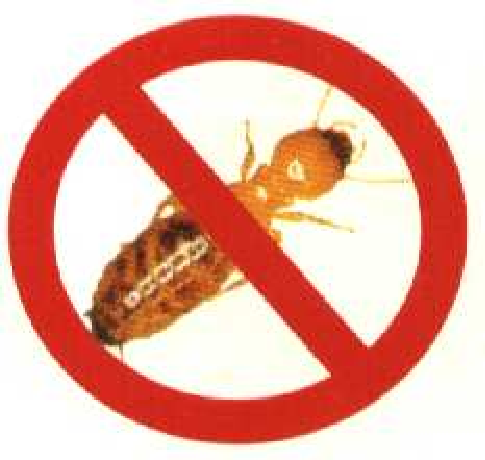
\includegraphics[width=0.5\textwidth]{Cap1/cupim}
%\caption{Proibido estacionar cupins. Legenda grande, com o objetivo de demonstrar a indenta��o na lista de figuras.}
%\label{cupim}
%\end{figure}

%\begin{table}
%\caption{Exemplo de uma Tabela}
%\label{minhatab}
%\center
%\begin{tabular}{cccc}
  % after \\: \hline or \cline{col1-col2} \cline{col3-col4} ...
 % \hline
%	Par�metro & Unidade & Valor da simula��o & Valor experimental   \\
%	\hline
 % Comprimento, $\alpha$ & $m$ &  $8,23$  & $8,54$ \\
 % Altura, $\beta$ & $m$     &  $29,1$ & $28,3$\\
%	Velocidade, $v$ & $m/s$  &  $60,2$ & $67,3$\\
%	\hline
%\end{tabular}
%\end{table}
